\PassOptionsToPackage{unicode=true}{hyperref} % options for packages loaded elsewhere
\PassOptionsToPackage{hyphens}{url}
%
\documentclass[10pt,xcolor=table,color={dvipsnames,usenames},ignorenonframetext,usepdftitle=false,french]{beamer}
\setbeamertemplate{caption}[numbered]
\setbeamertemplate{caption label separator}{: }
\setbeamercolor{caption name}{fg=normal text.fg}
\beamertemplatenavigationsymbolsempty
\usepackage{caption}
\captionsetup{skip=0pt,belowskip=0pt}
%\setlength\abovecaptionskip{-15pt}
\usepackage{lmodern}
\usepackage{amssymb,amsmath,mathtools,multirow}
\usepackage{float,hhline}
\usepackage{tikz}
\usepackage{mathtools}
\usepackage{ifxetex,ifluatex}
\usepackage{fixltx2e} % provides \textsubscript
\ifnum 0\ifxetex 1\fi\ifluatex 1\fi=0 % if pdftex
  \usepackage[T1]{fontenc}
  \usepackage[utf8]{inputenc}
  \usepackage{textcomp} % provides euro and other symbols
\else % if luatex or xelatex
  \usepackage{unicode-math}
  \defaultfontfeatures{Ligatures=TeX,Scale=MatchLowercase}
\fi
\usetheme[coding=utf8,language=english,
,titlepagelogo=img/logobeamer.png
]{TorinoTh}
% use upquote if available, for straight quotes in verbatim environments
\IfFileExists{upquote.sty}{\usepackage{upquote}}{}
% use microtype if available
\IfFileExists{microtype.sty}{%
\usepackage[]{microtype}
\UseMicrotypeSet[protrusion]{basicmath} % disable protrusion for tt fonts
}{}
\IfFileExists{parskip.sty}{%
\usepackage{parskip}
}{% else
\setlength{\parindent}{0pt}
\setlength{\parskip}{6pt plus 2pt minus 1pt}
}
\usepackage{hyperref}
\hypersetup{
            pdfauthor={Alain Quartier-la-Tente},
            pdfborder={0 0 0},
            breaklinks=true}
\urlstyle{same}  % don't use monospace font for urls
\newif\ifbibliography
\newlength{\cslhangindent}
\setlength{\cslhangindent}{1.5em}
\newlength{\csllabelwidth}
\setlength{\csllabelwidth}{3em}
\newenvironment{CSLReferences}[2] % #1 hanging-ident, #2 entry spacing
 {% don't indent paragraphs
  \setlength{\parindent}{0pt}
  % turn on hanging indent if param 1 is 1
  \ifodd #1 \everypar{\setlength{\hangindent}{\cslhangindent}}\ignorespaces\fi
  % set entry spacing
  \ifnum #2 > 0
  \setlength{\parskip}{#2\baselineskip}
  \fi
 }%
 {}
\usepackage{color}
\usepackage{fancyvrb}
\newcommand{\VerbBar}{|}
\newcommand{\VERB}{\Verb[commandchars=\\\{\}]}
\DefineVerbatimEnvironment{Highlighting}{Verbatim}{commandchars=\\\{\}}
% Add ',fontsize=\small' for more characters per line
\usepackage{framed}
\definecolor{shadecolor}{RGB}{248,248,248}
\newenvironment{Shaded}{\begin{snugshade}}{\end{snugshade}}
\newcommand{\AlertTok}[1]{\textcolor[rgb]{0.94,0.16,0.16}{#1}}
\newcommand{\AnnotationTok}[1]{\textcolor[rgb]{0.56,0.35,0.01}{\textbf{\textit{#1}}}}
\newcommand{\AttributeTok}[1]{\textcolor[rgb]{0.77,0.63,0.00}{#1}}
\newcommand{\BaseNTok}[1]{\textcolor[rgb]{0.00,0.00,0.81}{#1}}
\newcommand{\BuiltInTok}[1]{#1}
\newcommand{\CharTok}[1]{\textcolor[rgb]{0.31,0.60,0.02}{#1}}
\newcommand{\CommentTok}[1]{\textcolor[rgb]{0.56,0.35,0.01}{\textit{#1}}}
\newcommand{\CommentVarTok}[1]{\textcolor[rgb]{0.56,0.35,0.01}{\textbf{\textit{#1}}}}
\newcommand{\ConstantTok}[1]{\textcolor[rgb]{0.00,0.00,0.00}{#1}}
\newcommand{\ControlFlowTok}[1]{\textcolor[rgb]{0.13,0.29,0.53}{\textbf{#1}}}
\newcommand{\DataTypeTok}[1]{\textcolor[rgb]{0.13,0.29,0.53}{#1}}
\newcommand{\DecValTok}[1]{\textcolor[rgb]{0.00,0.00,0.81}{#1}}
\newcommand{\DocumentationTok}[1]{\textcolor[rgb]{0.56,0.35,0.01}{\textbf{\textit{#1}}}}
\newcommand{\ErrorTok}[1]{\textcolor[rgb]{0.64,0.00,0.00}{\textbf{#1}}}
\newcommand{\ExtensionTok}[1]{#1}
\newcommand{\FloatTok}[1]{\textcolor[rgb]{0.00,0.00,0.81}{#1}}
\newcommand{\FunctionTok}[1]{\textcolor[rgb]{0.00,0.00,0.00}{#1}}
\newcommand{\ImportTok}[1]{#1}
\newcommand{\InformationTok}[1]{\textcolor[rgb]{0.56,0.35,0.01}{\textbf{\textit{#1}}}}
\newcommand{\KeywordTok}[1]{\textcolor[rgb]{0.13,0.29,0.53}{\textbf{#1}}}
\newcommand{\NormalTok}[1]{#1}
\newcommand{\OperatorTok}[1]{\textcolor[rgb]{0.81,0.36,0.00}{\textbf{#1}}}
\newcommand{\OtherTok}[1]{\textcolor[rgb]{0.56,0.35,0.01}{#1}}
\newcommand{\PreprocessorTok}[1]{\textcolor[rgb]{0.56,0.35,0.01}{\textit{#1}}}
\newcommand{\RegionMarkerTok}[1]{#1}
\newcommand{\SpecialCharTok}[1]{\textcolor[rgb]{0.00,0.00,0.00}{#1}}
\newcommand{\SpecialStringTok}[1]{\textcolor[rgb]{0.31,0.60,0.02}{#1}}
\newcommand{\StringTok}[1]{\textcolor[rgb]{0.31,0.60,0.02}{#1}}
\newcommand{\VariableTok}[1]{\textcolor[rgb]{0.00,0.00,0.00}{#1}}
\newcommand{\VerbatimStringTok}[1]{\textcolor[rgb]{0.31,0.60,0.02}{#1}}
\newcommand{\WarningTok}[1]{\textcolor[rgb]{0.56,0.35,0.01}{\textbf{\textit{#1}}}}
\usepackage{graphicx,grffile}
\makeatletter
\def\maxwidth{\ifdim\Gin@nat@width>\linewidth\linewidth\else\Gin@nat@width\fi}
\def\maxheight{\ifdim\Gin@nat@height>\textheight\textheight\else\Gin@nat@height\fi}
\makeatother
% Scale images if necessary, so that they will not overflow the page
% margins by default, and it is still possible to overwrite the defaults
% using explicit options in \includegraphics[width, height, ...]{}
\setkeys{Gin}{width=\maxwidth,height=\maxheight,keepaspectratio}
% Prevent slide breaks in the middle of a paragraph:
\widowpenalties 1 10000
\raggedbottom
\AtBeginPart{
  \let\insertpartnumber\relax
  \let\partname\relax
  \frame{\partpage}
}
\AtBeginSection{
  \ifbibliography
  \else
    \begin{frame}[noframenumbering]{Contents}
    \tableofcontents[currentsection, hideothersubsections]
    \end{frame}
  \fi
}
\setlength{\emergencystretch}{3em}  % prevent overfull lines
\providecommand{\tightlist}{%
  %\setlength{\itemsep}{0pt}
  \setlength{\parskip}{0pt}
  }
\setcounter{secnumdepth}{0}

% set default figure placement to htbp
\makeatletter
\def\fps@figure{htbp}
\makeatother

\usepackage{dsfont}
\usepackage{stmaryrd}
\usepackage[normalem]{ulem}
\usepackage{fontawesome5}
\usepackage{tikz,pgfplots}
\pgfplotsset{compat=1.17}
\pgfplotsset{samples=100}
\usepackage{animate}
 \usepackage{booktabs}

\usepackage{colortbl}

\DeclareMathOperator{\Cov}{Cov}
\newcommand{\cov}[2]{\Cov\left( #1\,,\,#2 \right)}

\DeclareMathOperator{\e}{e}
\renewcommand{\P}{\mathds{P}} %Apparement \P existe déjà ?
\newcommand\N{\mathds{N}}
\newcommand\R{\mathds{R}}


\newcommand\1{\mathds{1}}
\newcommand{\E}[2][]{{\mathds{E}}_{#1}
  \def\temp{#2}\ifx\temp\empty
  \else
    \left[#2\right]
  \fi
}
\newcommand{\V}[2][]{{\mathds{V}}_{#1}
  \def\temp{#2}\ifx\temp\empty
  \else
    \left[#2\right]
  \fi
}
\newcommand\ud{\,\mathrm{d}}


% blocks
\usepackage{environ}
\usepackage[tikz]{bclogo}

\tikzstyle{titlestyle} =[draw=black!80,fill=black!20, text=black,
 right=10pt, rounded corners]
\mdfdefinestyle{symmaryboxstyle}{
	linecolor=black!80, backgroundcolor = black!5,
	skipabove=\baselineskip, innertopmargin=\baselineskip,
	innerbottommargin=\baselineskip,
	userdefinedwidth=\textwidth,
	middlelinewidth=1.2pt, roundcorner=5pt,
	skipabove={\dimexpr0.5\baselineskip+\topskip\relax},
	frametitleaboveskip=\dimexpr-\ht\strutbox\relax,
	innerlinewidth=0pt,
}
\NewEnviron{summary}{%
\begin{mdframed}[style=symmaryboxstyle]
\vspace{-0.5em}
\BODY
\end{mdframed}
}
\makeatletter
% Open `\noalign` and check for overlay specification:
\def\rowcolor{\noalign{\ifnum0=`}\fi\bmr@rowcolor}
\newcommand<>{\bmr@rowcolor}{%
    \alt#1%
        {\global\let\CT@do@color\CT@@do@color\@ifnextchar[\CT@rowa\CT@rowb}% Rest of original `\rowcolor`
        {\ifnum0=`{\fi}\@gooble@rowcolor}% End `\noalign` and gobble all arguments of `\rowcolor`.
}
% Gobble all normal arguments of `\rowcolor`:
\newcommand{\@gooble@rowcolor}[2][]{\@gooble@rowcolor@}
\newcommand{\@gooble@rowcolor@}[1][]{\@gooble@rowcolor@@}
\newcommand{\@gooble@rowcolor@@}[1][]{\ignorespaces}

\newcommand{\rowc}[1]{\only<#1>{\\\rowcolor{processblue!40}}}
%\newcommand{\rowc}[1]{{\rowcolor<#1>{processblue!30}}
\newcommand{\cellc}[1]{\only<#1>{\cellcolor{processblue!40}}}
\newcommand{\supsp}[1]{\visible<#1>{\\}}

\title{R and JDemetra+ 3.0:\\
A new toolbox around seasonal adjustment and time series analysis}
\ateneo{2\textsuperscript{nd}WS Time Series Methods for Official
Statistics}
\author{Alain Quartier-la-Tente}
\date{}


\setrellabel{}

\setcandidatelabel{}

\rel{}
\division{Insee\\
Session 10: Seasonal and Calendar Adjustment}

\departement{Friday 23 September 2022}
\makeatletter
\let\@@magyar@captionfix\relax
\makeatother


\begin{document}
\begin{frame}[plain,noframenumbering]
\titlepage
\end{frame}

\hypertarget{introduction}{%
\section{Introduction}\label{introduction}}

\begin{frame}[fragile]{Introduction (1)}
\protect\hypertarget{introduction-1}{}
\begin{itemize}
\item
  In March 2019, \texttt{RJDemetra} was published on CRAN:

  \begin{itemize}
  \item
    first \faIcon{r-project} package that enables to use TRAMO-SEATS
  \item
    faster than existing \faIcon{r-project} packages on seasonal
    adjustment
  \item
    enables to interact with JDemetra+ ``workspaces'' used in production
  \end{itemize}
\end{itemize}

\pause

\begin{itemize}
\tightlist
\item
  With the development of JDemetra+ 3.0, more than 13 \faIcon{r-project}
  packages are being developped! Not only on seasonal adjustment!
\end{itemize}

\pause

\begin{itemize}
\tightlist
\item
  They are require Java \faIcon{java} \(\geq\) 17 (see for example
  installation manual of \texttt{RJDemetra}:
  \url{https://github.com/jdemetra/rjdemetra/wiki/Installation-manual})
\end{itemize}
\end{frame}

\begin{frame}[fragile]{Introduction (2)}
\protect\hypertarget{introduction-2}{}
They are all available in GitHub, currently:

\begin{Shaded}
\begin{Highlighting}[]
\CommentTok{\# install.packages("remotes")}
\NormalTok{remotes}\SpecialCharTok{::}\FunctionTok{install\_github}\NormalTok{(}\StringTok{"palatej/rjd3toolkit"}\NormalTok{)}
\NormalTok{remotes}\SpecialCharTok{::}\FunctionTok{install\_github}\NormalTok{(}\StringTok{"palatej/rjd3modelling"}\NormalTok{)}
\NormalTok{remotes}\SpecialCharTok{::}\FunctionTok{install\_github}\NormalTok{(}\StringTok{"palatej/rjd3sa"}\NormalTok{)}
\NormalTok{remotes}\SpecialCharTok{::}\FunctionTok{install\_github}\NormalTok{(}\StringTok{"palatej/rjd3arima"}\NormalTok{)}
\NormalTok{remotes}\SpecialCharTok{::}\FunctionTok{install\_github}\NormalTok{(}\StringTok{"palatej/rjd3x13"}\NormalTok{)}
\NormalTok{remotes}\SpecialCharTok{::}\FunctionTok{install\_github}\NormalTok{(}\StringTok{"palatej/rjd3tramoseats"}\NormalTok{)}
\NormalTok{remotes}\SpecialCharTok{::}\FunctionTok{install\_github}\NormalTok{(}\StringTok{"palatej/rjdemetra3"}\NormalTok{)}
\NormalTok{remotes}\SpecialCharTok{::}\FunctionTok{install\_github}\NormalTok{(}\StringTok{"palatej/rjdfilters"}\NormalTok{)}
\NormalTok{remotes}\SpecialCharTok{::}\FunctionTok{install\_github}\NormalTok{(}\StringTok{"palatej/rjd3sts"}\NormalTok{)}
\NormalTok{remotes}\SpecialCharTok{::}\FunctionTok{install\_github}\NormalTok{(}\StringTok{"palatej/rjd3highfreq"}\NormalTok{)}
\NormalTok{remotes}\SpecialCharTok{::}\FunctionTok{install\_github}\NormalTok{(}\StringTok{"palatej/rjd3stl"}\NormalTok{)}
\NormalTok{remotes}\SpecialCharTok{::}\FunctionTok{install\_github}\NormalTok{(}\StringTok{"palatej/rjd3bench"}\NormalTok{)}
\NormalTok{remotes}\SpecialCharTok{::}\FunctionTok{install\_github}\NormalTok{(}\StringTok{"AQLT/ggdemetra3"}\NormalTok{)}
\end{Highlighting}
\end{Shaded}
\end{frame}

\begin{frame}{Introduction (3)}
\protect\hypertarget{introduction-3}{}
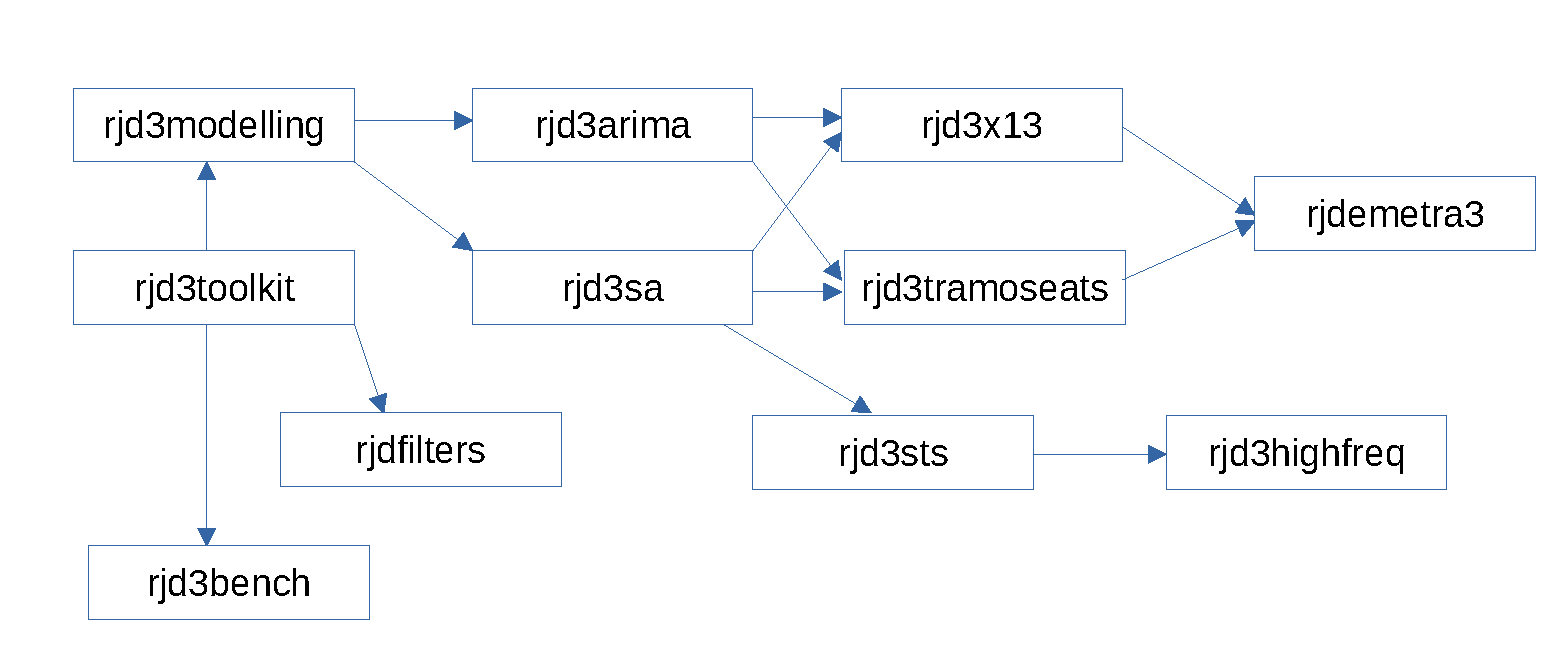
\includegraphics{img/diag.pdf}

And it's just the begining!
\end{frame}

\hypertarget{utility-packages}{%
\section{Utility packages}\label{utility-packages}}

\hypertarget{rjd3toolkit}{%
\subsection{rjd3toolkit}\label{rjd3toolkit}}

\begin{frame}[fragile]{rjd3toolkit}
\protect\hypertarget{rjd3toolkit-1}{}
Contains several utility functions used in other \texttt{rjd} packages
and several functions to perform tests:

\begin{itemize}
\item
  Normality tests: Bowman-Shenton (\texttt{bowmanshenton()}),
  Doornik-Hansen (\texttt{doornikhansen()}), Jarque-Bera
  (\texttt{jarquebera()})
\item
  \bclampe Runs tests (randomness of data): mean or the median
  (\texttt{testofruns()}) or up and down runs test
  (\texttt{testofupdownruns()})
\item
  autocorrelation functions (usual, inverse, partial)
\item
  \texttt{aggregate()} to aggregate a time serie to a higher frequency
\end{itemize}
\end{frame}

\begin{frame}[fragile,allowframebreaks]{Examples}
\protect\hypertarget{examples}{}
\footnotesize

\begin{Shaded}
\begin{Highlighting}[]
\FunctionTok{library}\NormalTok{(rjd3toolkit)}
\FunctionTok{set.seed}\NormalTok{(}\DecValTok{100}\NormalTok{)}
\NormalTok{x }\OtherTok{=} \FunctionTok{rnorm}\NormalTok{(}\DecValTok{1000}\NormalTok{);y }\OtherTok{=} \FunctionTok{rlnorm}\NormalTok{(}\DecValTok{1000}\NormalTok{)}
\FunctionTok{bowmanshenton}\NormalTok{(x) }\CommentTok{\# normal distribution}
\end{Highlighting}
\end{Shaded}

\begin{verbatim}
## Value:  0.3117551 
## P-Value:  0.8557
\end{verbatim}

\begin{Shaded}
\begin{Highlighting}[]
\FunctionTok{bowmanshenton}\NormalTok{(y) }\CommentTok{\# log{-}normal distribution}
\end{Highlighting}
\end{Shaded}

\begin{verbatim}
## Value:  33551.78 
## P-Value:  0.0000
\end{verbatim}

\begin{Shaded}
\begin{Highlighting}[]
\FunctionTok{testofruns}\NormalTok{(x) }\CommentTok{\# random data}
\end{Highlighting}
\end{Shaded}

\begin{verbatim}
## Value:  1.396856 
## P-Value:  0.1625
\end{verbatim}

\begin{Shaded}
\begin{Highlighting}[]
\FunctionTok{testofruns}\NormalTok{(y) }\CommentTok{\# random data}
\end{Highlighting}
\end{Shaded}

\begin{verbatim}
## Value:  -0.1150397 
## P-Value:  0.9084
\end{verbatim}

\begin{Shaded}
\begin{Highlighting}[]
\FunctionTok{testofruns}\NormalTok{(}\DecValTok{1}\SpecialCharTok{:}\DecValTok{1000}\NormalTok{) }\CommentTok{\# non{-}random data}
\end{Highlighting}
\end{Shaded}

\begin{verbatim}
## Value:  -31.57534 
## P-Value:  0.0000
\end{verbatim}

\begin{Shaded}
\begin{Highlighting}[]
\FunctionTok{autocorrelations}\NormalTok{(x)}
\end{Highlighting}
\end{Shaded}

\begin{verbatim}
##            1            2            3            4 
## -0.039797636 -0.028616535  0.038409192  0.012282902 
##            5            6            7            8 
## -0.035815187 -0.008406605  0.010077238  0.037414192 
##            9           10           11           12 
## -0.063957619 -0.015995017 -0.003748914  0.016326224 
##           13           14           15 
## -0.051273264 -0.015552059  0.035965008
\end{verbatim}

\begin{Shaded}
\begin{Highlighting}[]
\FunctionTok{autocorrelations.inverse}\NormalTok{(x)}
\end{Highlighting}
\end{Shaded}

\begin{verbatim}
##            1            2            3            4 
## -0.038225207 -0.030030005  0.034985887  0.014697477 
##            5            6            7            8 
## -0.032164035 -0.012375939  0.005587471  0.039725092 
##            9           10           11           12 
## -0.057199640 -0.020771981 -0.011968366  0.019437797 
##           13           14           15 
## -0.043170872 -0.021167341  0.027156206
\end{verbatim}

\begin{Shaded}
\begin{Highlighting}[]
\FunctionTok{autocorrelations.partial}\NormalTok{(x)}
\end{Highlighting}
\end{Shaded}

\begin{verbatim}
##            1            2            3            4 
## -0.039797636 -0.030248296  0.036122272  0.014485158 
##            5            6            7            8 
## -0.032734128 -0.011864534  0.006444671  0.040137674 
##            9           10           11           12 
## -0.059177846 -0.020600211 -0.012229212  0.019298100 
##           13           14           15 
## -0.045255005 -0.021485597  0.028314840
\end{verbatim}
\end{frame}

\hypertarget{rjd3modelling}{%
\subsection{rjd3modelling}\label{rjd3modelling}}

\begin{frame}[fragile]{rjd3modelling}
\protect\hypertarget{rjd3modelling-1}{}
\begin{itemize}
\item
  \bclampe create user-defined calendar and trading-days regressors:
  \texttt{calendar.new()} (create a new calendar),
  \texttt{calendar.holiday()} (add a specific holiday, e.g.~christmas),
  \texttt{calendar.easter()} (easter related day) and
  \texttt{calendar.fixedday()})
\item
  \bclampe create outliers regressors (AO, LS, TC, SO, Ramp,
  intervention variables), calendar related regressors (stock, leap
  year, periodic dummies and contrasts, trigonometric variables)
  -\textgreater{} to be added quadratic ramps
\item
  \bclampe  Range-mean regression test (to choose log transformation),
  Canova-Hansen (\texttt{td.ch()}) and trading-days f-test
  (\texttt{td.f()})
\item
  specification functions for \texttt{rjd3x13} and
  \texttt{rjd3tramoseats}
\end{itemize}
\end{frame}

\begin{frame}[fragile,allowframebreaks]{Example of a specific calendar}
\protect\hypertarget{example-of-a-specific-calendar}{}
\begin{Shaded}
\begin{Highlighting}[]
\FunctionTok{library}\NormalTok{(rjd3modelling)}
\NormalTok{fr\_cal }\OtherTok{\textless{}{-}} \FunctionTok{calendar.new}\NormalTok{()}
\FunctionTok{calendar.holiday}\NormalTok{(fr\_cal, }\StringTok{"NEWYEAR"}\NormalTok{)}
\FunctionTok{calendar.holiday}\NormalTok{(fr\_cal, }\StringTok{"EASTERMONDAY"}\NormalTok{)}
\FunctionTok{calendar.holiday}\NormalTok{(fr\_cal, }\StringTok{"MAYDAY"}\NormalTok{)}
\FunctionTok{calendar.fixedday}\NormalTok{(fr\_cal, }\AttributeTok{month =} \DecValTok{5}\NormalTok{, }\AttributeTok{day =} \DecValTok{8}\NormalTok{,}
                  \AttributeTok{start =} \StringTok{"1953{-}03{-}20"}\NormalTok{)}
\CommentTok{\# calendar.holiday(fr\_cal, "WHITMONDAY") \# Equivalent to:}
\FunctionTok{calendar.easter}\NormalTok{(fr\_cal, }\AttributeTok{offset =} \DecValTok{61}\NormalTok{)}

\FunctionTok{calendar.fixedday}\NormalTok{(fr\_cal, }\AttributeTok{month =} \DecValTok{7}\NormalTok{, }\AttributeTok{day =} \DecValTok{14}\NormalTok{)}
\CommentTok{\# calendar.holiday(fr\_cal, "ASSUMPTION")}
\FunctionTok{calendar.easter}\NormalTok{(fr\_cal, }\AttributeTok{offset =} \DecValTok{61}\NormalTok{)}
\FunctionTok{calendar.holiday}\NormalTok{(fr\_cal, }\StringTok{"ALLSAINTSDAY"}\NormalTok{)}
\FunctionTok{calendar.holiday}\NormalTok{(fr\_cal, }\StringTok{"ARMISTICE"}\NormalTok{)}
\FunctionTok{calendar.holiday}\NormalTok{(fr\_cal, }\StringTok{"CHRISTMAS"}\NormalTok{)}
\end{Highlighting}
\end{Shaded}

\footnotesize

Use \texttt{holidays()} to get the days of the holidays and
\texttt{htd()} to get the trading days regressors

\begin{Shaded}
\begin{Highlighting}[]
\FunctionTok{holidays}\NormalTok{(fr\_cal, }\StringTok{"2020{-}12{-}24"}\NormalTok{, }\DecValTok{10}\NormalTok{,}\AttributeTok{single =}\NormalTok{ T)}
\end{Highlighting}
\end{Shaded}

\begin{verbatim}
##            [,1]
## 2020-12-24    0
## 2020-12-25    1
## 2020-12-26    0
## 2020-12-27    0
## 2020-12-28    0
## 2020-12-29    0
## 2020-12-30    0
## 2020-12-31    0
## 2021-01-01    1
## 2021-01-02    0
\end{verbatim}

\begin{Shaded}
\begin{Highlighting}[]
\NormalTok{s }\OtherTok{=} \FunctionTok{ts}\NormalTok{(}\DecValTok{0}\NormalTok{, }\AttributeTok{start =} \DecValTok{2020}\NormalTok{, }\AttributeTok{end =} \FunctionTok{c}\NormalTok{(}\DecValTok{2020}\NormalTok{, }\DecValTok{11}\NormalTok{), }\AttributeTok{frequency =} \DecValTok{12}\NormalTok{)}
\CommentTok{\# Trading{-}days regressors (each day has a different effect, sunday as contrasts)}
\NormalTok{td\_reg }\OtherTok{\textless{}{-}} \FunctionTok{htd}\NormalTok{(fr\_cal, }\AttributeTok{s =}\NormalTok{ s, }\AttributeTok{groups =} \FunctionTok{c}\NormalTok{(}\DecValTok{1}\NormalTok{, }\DecValTok{2}\NormalTok{, }\DecValTok{3}\NormalTok{, }\DecValTok{4}\NormalTok{, }\DecValTok{5}\NormalTok{, }\DecValTok{6}\NormalTok{, }\DecValTok{0}\NormalTok{))}
\CommentTok{\# Working{-}days regressors (Monday = ... = Friday; Saturday = Sunday = contrasts)}
\NormalTok{wd\_reg }\OtherTok{\textless{}{-}} \FunctionTok{htd}\NormalTok{(fr\_cal, }\AttributeTok{s =}\NormalTok{ s, }\AttributeTok{groups =} \FunctionTok{c}\NormalTok{(}\DecValTok{1}\NormalTok{, }\DecValTok{1}\NormalTok{, }\DecValTok{1}\NormalTok{, }\DecValTok{1}\NormalTok{, }\DecValTok{1}\NormalTok{, }\DecValTok{0}\NormalTok{, }\DecValTok{0}\NormalTok{))}
\CommentTok{\# Monday = ... = Friday; Saturday; Sunday = contrasts}
\NormalTok{wd\_reg }\OtherTok{\textless{}{-}} \FunctionTok{htd}\NormalTok{(fr\_cal, }\AttributeTok{s =}\NormalTok{ s, }\AttributeTok{groups =} \FunctionTok{c}\NormalTok{(}\DecValTok{1}\NormalTok{, }\DecValTok{1}\NormalTok{, }\DecValTok{1}\NormalTok{, }\DecValTok{1}\NormalTok{, }\DecValTok{1}\NormalTok{, }\DecValTok{2}\NormalTok{, }\DecValTok{0}\NormalTok{))}
\NormalTok{wd\_reg}
\end{Highlighting}
\end{Shaded}

\begin{verbatim}
##             group-1    group-2
## Jan 2020  2.0000000  0.0000000
## Feb 2020  0.0000000  1.0000000
## Mar 2020 -1.7809251 -0.7968209
## Apr 2020  0.7809251 -0.2031791
## May 2020 -3.1554920  0.4740847
## Jun 2020  5.1554920  0.5259153
## Jul 2020  2.0000000  0.0000000
## Aug 2020 -4.0000000  0.0000000
## Sep 2020  2.0000000  0.0000000
## Oct 2020  2.0000000  1.0000000
## Nov 2020  0.0000000  0.0000000
\end{verbatim}
\end{frame}

\begin{frame}[fragile,allowframebreaks]{Example of outliers}
\protect\hypertarget{example-of-outliers}{}
\footnotesize

\begin{Shaded}
\begin{Highlighting}[]
\NormalTok{s }\OtherTok{=} \FunctionTok{ts}\NormalTok{(}\DecValTok{0}\NormalTok{, }\AttributeTok{start =} \DecValTok{2000}\NormalTok{, }\AttributeTok{end =} \DecValTok{2005}\NormalTok{, }\AttributeTok{frequency =} \DecValTok{12}\NormalTok{)}
\NormalTok{ao }\OtherTok{=} \FunctionTok{ao.variable}\NormalTok{(}\AttributeTok{s =}\NormalTok{ s, }\AttributeTok{date =} \StringTok{"2001{-}03{-}01"}\NormalTok{)}
\NormalTok{ls }\OtherTok{=} \FunctionTok{ls.variable}\NormalTok{(}\AttributeTok{s =}\NormalTok{ s, }\AttributeTok{date =} \StringTok{"2001{-}01{-}01"}\NormalTok{)}
\NormalTok{tc }\OtherTok{=} \FunctionTok{tc.variable}\NormalTok{(}\AttributeTok{s =}\NormalTok{ s, }\AttributeTok{date =} \StringTok{"2001{-}01{-}01"}\NormalTok{, }\AttributeTok{rate =} \FloatTok{0.7}\NormalTok{)}
\NormalTok{so }\OtherTok{=} \FunctionTok{so.variable}\NormalTok{(}\AttributeTok{s =}\NormalTok{ s, }\AttributeTok{date =} \StringTok{"2003{-}05{-}01"}\NormalTok{)}
\NormalTok{ramp }\OtherTok{=} \FunctionTok{ramp.variable}\NormalTok{(}\AttributeTok{s =}\NormalTok{ s, }\AttributeTok{range =} \FunctionTok{c}\NormalTok{(}\StringTok{"2001{-}01{-}01"}\NormalTok{,}\StringTok{"2001{-}12{-}01"}\NormalTok{))}
\FunctionTok{plot}\NormalTok{(}\FunctionTok{ts.union}\NormalTok{(ao, ls, tc, so, ramp), }\AttributeTok{plot.type =} \StringTok{"single"}\NormalTok{,}
     \AttributeTok{col =} \FunctionTok{c}\NormalTok{(}\StringTok{"red"}\NormalTok{,}\StringTok{"lightgreen"}\NormalTok{,}\StringTok{"orange"}\NormalTok{,}\StringTok{"blue"}\NormalTok{,}\StringTok{"black"}\NormalTok{))}
\end{Highlighting}
\end{Shaded}

\begin{center}\includegraphics{img/markdown-outplot-1} \end{center}
\end{frame}

\hypertarget{rjd3sa}{%
\subsection{rjd3sa}\label{rjd3sa}}

\begin{frame}[fragile]{rjd3sa (1)}
\protect\hypertarget{rjd3sa-1}{}
Seasonality tests:

\begin{itemize}
\item
  Canova-Hansen (\texttt{seasonality.canovahansen()})
\item
  \bclampe X-12 combined test (\texttt{seasonality.combined()})
\item
  F-test on seasonal dummies (\texttt{seasonality.f()})
\item
  Friedman Seasonality Test (\texttt{seasonality.friedman()})
\item
  Kruskall-Wallis Seasonality Test
  (\texttt{seasonality.kruskalwallis()})
\item
  \bclampe Periodogram Seasonality Test
  (\texttt{seasonality.periodogram()})
\item
  QS Seasonality Test (\texttt{seasonality.qs()})
\end{itemize}
\end{frame}

\begin{frame}[fragile]{rjd3sa (2)}
\protect\hypertarget{rjd3sa-2}{}
\bcattention Always correct the trend and remove the mean before
seasonality tests: \footnotesize

\begin{Shaded}
\begin{Highlighting}[]
\FunctionTok{library}\NormalTok{(rjd3sa)}
\NormalTok{y }\OtherTok{=} \FunctionTok{diff}\NormalTok{(rjd3toolkit}\SpecialCharTok{::}\NormalTok{ABS}\SpecialCharTok{$}\NormalTok{X0.}\DecValTok{2}\NormalTok{.}\DecValTok{09}\NormalTok{.}\FloatTok{10.}\NormalTok{M, }\DecValTok{1}\NormalTok{); y }\OtherTok{=}\NormalTok{ y }\SpecialCharTok{{-}} \FunctionTok{mean}\NormalTok{(y)}
\FunctionTok{seasonality.f}\NormalTok{(y, }\DecValTok{12}\NormalTok{)}
\end{Highlighting}
\end{Shaded}

\begin{verbatim}
## Value:  378.9234 
## P-Value:  0.0000
\end{verbatim}

\begin{Shaded}
\begin{Highlighting}[]
\FunctionTok{seasonality.friedman}\NormalTok{(y, }\DecValTok{12}\NormalTok{)}
\end{Highlighting}
\end{Shaded}

\begin{verbatim}
## Value:  298.2529 
## P-Value:  0.0000
\end{verbatim}

\begin{Shaded}
\begin{Highlighting}[]
\FunctionTok{seasonality.kruskalwallis}\NormalTok{(y, }\DecValTok{12}\NormalTok{)}
\end{Highlighting}
\end{Shaded}

\begin{verbatim}
## Value:  319.9801 
## P-Value:  0.0000
\end{verbatim}

\begin{Shaded}
\begin{Highlighting}[]
\FunctionTok{seasonality.combined}\NormalTok{(y, }\DecValTok{12}\NormalTok{)}
\end{Highlighting}
\end{Shaded}

\begin{verbatim}
## $seasonality
## [1] "PRESENT"
## 
## $kruskalwallis
## $kruskalwallis$value
## [1] 319.9801
## 
## $kruskalwallis$pvalue
## [1] 0
## 
## $kruskalwallis$description
## [1] "Chi2 with 11.0 degrees of freedom "
## 
## 
## $stable
## $stable$SSM
## [1] 69596527
## 
## $stable$dfM
## [1] 11
## 
## $stable$SSR
## [1] 6721009
## 
## $stable$dfR
## [1] 412
## 
## $stable$test
## Value:  387.8445 
## P-Value:  0.0000 
## 
## 
## $evolutive
## $evolutive$SSM
## [1] 2145849
## 
## $evolutive$dfM
## [1] 34
## 
## $evolutive$SSR
## [1] 3800578
## 
## $evolutive$dfR
## [1] 374
## 
## $evolutive$test
## Value:  6.210723 
## P-Value:  0.0000
\end{verbatim}
\end{frame}

\hypertarget{seasonal-adjustment-packages}{%
\section{Seasonal adjustment
packages}\label{seasonal-adjustment-packages}}

\hypertarget{rjd3arima}{%
\subsection{rjd3arima}\label{rjd3arima}}

\begin{frame}[fragile]{rjd3arima}
\protect\hypertarget{rjd3arima-1}{}
\texttt{rjd3arima} is devoted to formatting the output of Arima related
results
\end{frame}

\hypertarget{rjd3x13-and-rjd3tramoseats}{%
\subsection{rjd3x13 and
rjd3tramoseats}\label{rjd3x13-and-rjd3tramoseats}}

\begin{frame}[fragile]{Common functions}
\protect\hypertarget{common-functions}{}
In \texttt{RJDemetra} you have one function to set the specification
(\texttt{regarima\_spec\_x13()}, \texttt{regarima\_spec\_tramo()},
\texttt{x13\_spec()} and \texttt{tramoseats\_spec()}) now one function
for each part of the specification

\pause

Common functions (defined in \texttt{rjd3modelling}) to set the
specification of the preprocessing:

\texttt{set\_arima()}, \texttt{set\_automodel()}, \texttt{set\_basic()},
\texttt{set\_easter()}, \texttt{set\_estimate()},
\texttt{set\_outlier()}, \texttt{set\_tradingdays()},
\texttt{set\_transform()}, \texttt{add\_outlier()} and
\texttt{remove\_outlier()}, \texttt{add\_ramp()} and
\texttt{remove}\_ramp()`

\bcinterdit \texttt{add\_usrdefvar()} not yet available
\end{frame}

\begin{frame}[fragile]{rjd3x13}
\protect\hypertarget{rjd3x13}{}
Main functions:

\begin{itemize}
\item
  Specification: created with \texttt{spec\_x11\_default()},
  \texttt{spec\_x13\_default()}, \texttt{spec\_regarima\_default()} and
  customized with \texttt{rjd3arima} functions + \texttt{set\_x11()}
\item
  Apply model with \texttt{x11()}, \texttt{x13()}, \texttt{fast.x13()},
  \texttt{regarima()}, \texttt{fast.regarima()}
\item
  \bclampe Refresh policies: \texttt{regarima.refresh()} and
  \texttt{x13.refresh()}
\end{itemize}
\end{frame}

\begin{frame}{Performance}
\protect\hypertarget{performance}{}
\begin{center}\includegraphics[height=0.9\textheight]{img/markdown-performance-1} \end{center}
\end{frame}

\begin{frame}[fragile,allowframebreaks]{Exemple}
\protect\hypertarget{exemple}{}
\footnotesize

\begin{Shaded}
\begin{Highlighting}[]
\FunctionTok{library}\NormalTok{(rjd3modelling);}\FunctionTok{library}\NormalTok{(rjd3x13)}
\NormalTok{y }\OtherTok{=}\NormalTok{ rjd3toolkit}\SpecialCharTok{::}\NormalTok{ABS}\SpecialCharTok{$}\NormalTok{X0.}\DecValTok{2}\NormalTok{.}\DecValTok{09}\NormalTok{.}\FloatTok{10.}\NormalTok{M}
\NormalTok{spec }\OtherTok{=} \FunctionTok{spec\_x13\_default}\NormalTok{(}\StringTok{"rsa5c"}\NormalTok{) }\SpecialCharTok{|\textgreater{}} \FunctionTok{set\_easter}\NormalTok{(}\AttributeTok{type =} \StringTok{"unused"}\NormalTok{) }\SpecialCharTok{|\textgreater{}} 
  \FunctionTok{set\_outlier}\NormalTok{(}\AttributeTok{outliers.type =} \FunctionTok{c}\NormalTok{(}\StringTok{"AO"}\NormalTok{, }\StringTok{"LS"}\NormalTok{)) }\SpecialCharTok{|\textgreater{}} 
  \FunctionTok{set\_tradingdays}\NormalTok{(}\AttributeTok{test =} \StringTok{"None"}\NormalTok{) }\SpecialCharTok{|\textgreater{}} \FunctionTok{set\_x11}\NormalTok{(}\AttributeTok{henderson.filter =} \DecValTok{13}\NormalTok{) }\SpecialCharTok{|\textgreater{}} 
  \FunctionTok{add\_outlier}\NormalTok{(}\AttributeTok{type =} \StringTok{"TC"}\NormalTok{, }\AttributeTok{date =} \StringTok{"2000{-}06{-}01"}\NormalTok{,}
              \AttributeTok{name =} \StringTok{"My TC in 2000{-}06"}\NormalTok{) }
\NormalTok{m }\OtherTok{=}\NormalTok{ rjd3x13}\SpecialCharTok{::}\FunctionTok{fast.x13}\NormalTok{(y, spec)}
\CommentTok{\# m is a list with several outputs:}
\FunctionTok{names}\NormalTok{(m)}
\end{Highlighting}
\end{Shaded}

\begin{verbatim}
## [1] "preprocessing" "preadjust"     "decomposition"
## [4] "final"         "mstats"        "diagnostics"  
## [7] "user_defined"
\end{verbatim}

\begin{Shaded}
\begin{Highlighting}[]
\NormalTok{m}
\end{Highlighting}
\end{Shaded}

\begin{verbatim}
## RegARIMA
## Log-transformation: yes 
## SARIMA model:  (0,1,2) (1,1,1) 
## 
## Coefficients
##           Estimate Std. Error  T-stat
## theta(1)  -1.01804    0.07639 -13.326
## theta(2)   0.20863    0.05378   3.879
## bphi(1)   -0.26680    0.05399  -4.942
## btheta(1) -0.77559    0.05384 -14.405
## 
## Regression model:
##                   Estimate Std. Error T-stat
## monday           -0.011247   0.004004 -2.809
## tuesday           0.005870   0.004013  1.463
## wednesday        -0.002002   0.004003 -0.500
## thursday          0.014483   0.004021  3.602
## friday            0.001577   0.004023  0.392
## saturday          0.011465   0.003996  2.869
## lp                0.037501   0.010994  3.411
## easter            0.053486   0.008319  6.429
## My TC in 2000-06  0.022947   0.023666  0.970
## Number of observations:  425 
## Number of effective observations:  412 
## Number of parameters:  14 
## 
## Loglikelihood:  763.5143 
## Adjusted loglikelihood:  -2104.113 
## 
## Standard error of the regression (ML estimate):  0.03757223 
## AIC:  4236.225 
## AICC:  4237.283 
## BIC:  4292.519 
## 
## 
## Decomposition
## Monitoring and Quality Assessment Statistics: 
##     M stats
## m1    0.045
## m2    0.043
## m3    1.778
## m4    0.403
## m5    1.419
## m6    0.020
## m7    0.052
## m8    0.155
## m9    0.049
## m10   0.116
## m11   0.112
## q     0.410
## qm2   0.455
## 
## Final filters: 
## Seasonal filter:  
## Trend filter: 13 terms Henderson moving average
## 
## Diagnostics
## Relative contribution of the components to the stationary
## portion of the variance in the original series,
## after the removal of the long term trend (in %)
## 
##            Component
##  cycle        13.508
##  seasonal     86.645
##  irregular     0.429
##  calendar      0.688
##  others        0.004
##  total       101.274
## 
## Residual seasonality tests
##                 P.value
##  seas.ftest.i     0.975
##  seas.ftest.sa    0.999
##  seas.qstest.i    0.984
##  seas.qstest.sa   1.000
##  td.ftest.i       0.982
##  td.ftest.sa      0.982
## 
## 
## Final
## Last values
##          series       sa    trend seas       irr
## Sep 2016 1393.5 1537.129 1537.064    1 1.0000420
## Oct 2016 1497.4 1588.929 1531.988    1 1.0371684
## Nov 2016 1684.3 1520.076 1532.076    1 0.9921677
## Dec 2016 2850.4 1535.647 1537.080    1 0.9990677
## Jan 2017 1428.5 1547.286 1544.701    1 1.0016735
## Feb 2017 1092.4 1547.740 1552.749    1 0.9967744
## Mar 2017 1370.3 1554.062 1557.995    1 0.9974762
## Apr 2017 1522.6 1588.035 1557.819    1 1.0193965
## May 2017 1452.4 1556.976 1553.193    1 1.0024353
## Jun 2017 1557.2 1533.334 1546.419    1 0.9915389
## Jul 2017 1445.5 1535.987 1540.819    1 0.9968643
## Aug 2017 1303.1 1518.261 1537.522    1 0.9874725
\end{verbatim}

\begin{Shaded}
\begin{Highlighting}[]
\FunctionTok{summary}\NormalTok{(m}\SpecialCharTok{$}\NormalTok{preprocessing)}
\end{Highlighting}
\end{Shaded}

\begin{verbatim}
## Log-transformation: yes 
## SARIMA model:  (0,1,2) (1,1,1) 
## 
## Coefficients
##           Estimate Std. Error  T-stat Pr(>|t|)    
## theta(1)  -1.01804    0.07639 -13.326  < 2e-16 ***
## theta(2)   0.20863    0.05378   3.879 0.000123 ***
## bphi(1)   -0.26680    0.05399  -4.942 1.14e-06 ***
## btheta(1) -0.77559    0.05384 -14.405  < 2e-16 ***
## ---
## Signif. codes:  
## 0 '***' 0.001 '**' 0.01 '*' 0.05 '.' 0.1 ' ' 1
## 
## Regression model:
##                   Estimate Std. Error T-stat Pr(>|t|)    
## monday           -0.011247   0.004004 -2.809 0.005219 ** 
## tuesday           0.005870   0.004013  1.463 0.144306    
## wednesday        -0.002002   0.004003 -0.500 0.617304    
## thursday          0.014483   0.004021  3.602 0.000356 ***
## friday            0.001577   0.004023  0.392 0.695391    
## saturday          0.011465   0.003996  2.869 0.004333 ** 
## lp                0.037501   0.010994  3.411 0.000713 ***
## easter            0.053486   0.008319  6.429 3.67e-10 ***
## My TC in 2000-06  0.022947   0.023666  0.970 0.332814    
## ---
## Signif. codes:  
## 0 '***' 0.001 '**' 0.01 '*' 0.05 '.' 0.1 ' ' 1
## Number of observations:  425 , Number of effective observations:  412 , Number of parameters:  14 
## Loglikelihood:  763.5143, Adjusted loglikelihood:  -2104.113
## Standard error of the regression (ML estimate):  0.03757223 
## AIC:  4236.225 , AICc:  4237.283 , BIC:  4292.519
\end{verbatim}

\begin{Shaded}
\begin{Highlighting}[]
\FunctionTok{plot}\NormalTok{(m)}
\end{Highlighting}
\end{Shaded}

\begin{center}\includegraphics[height=0.5\textheight]{img/markdown-x13-1} \end{center}
\end{frame}

\hypertarget{rjd3tramoseats}{%
\subsection{rjd3tramoseats}\label{rjd3tramoseats}}

\begin{frame}[fragile]{rjd3tramoseats}
\protect\hypertarget{rjd3tramoseats-1}{}
Main functions:

\begin{itemize}
\item
  Specification: created with \texttt{spec\_tramoseats\_default()},
  \texttt{spec\_tramo\_default()} and customized with \texttt{rjd3arima}
  functions + \texttt{set\_seats()}
\item
  Apply model with \texttt{tramoseats()}, \texttt{fast.tramoseats()},
  \texttt{tramo()}, \texttt{fast.tramo()}
\item
  \bclampe Refresh policies: \texttt{tramo.refresh()} and
  \texttt{tramoseats.refresh()}
\end{itemize}
\end{frame}

\begin{frame}[fragile,allowframebreaks]{Exemple}
\protect\hypertarget{exemple-1}{}
\footnotesize

\begin{Shaded}
\begin{Highlighting}[]
\NormalTok{spec }\OtherTok{=} \FunctionTok{spec\_tramoseats\_default}\NormalTok{(}\StringTok{"rsafull"}\NormalTok{) }\SpecialCharTok{|\textgreater{}} 
  \FunctionTok{set\_easter}\NormalTok{(}\AttributeTok{type =} \StringTok{"IncludeEasterMonday"}\NormalTok{) }\SpecialCharTok{|\textgreater{}} 
  \FunctionTok{set\_tradingdays}\NormalTok{(}\AttributeTok{test =} \StringTok{"Separate\_T"}\NormalTok{) }\SpecialCharTok{|\textgreater{}} 
  \FunctionTok{set\_seats}\NormalTok{(}\AttributeTok{algorithm =} \StringTok{"KalmanSmoother"}\NormalTok{)}
\NormalTok{m }\OtherTok{=}\NormalTok{ rjd3tramoseats}\SpecialCharTok{::}\FunctionTok{tramoseats}\NormalTok{(y, spec)}
\CommentTok{\# More informations:}
\FunctionTok{names}\NormalTok{(m)}
\end{Highlighting}
\end{Shaded}

\begin{verbatim}
## [1] "result"          "estimation_spec" "result_spec"    
## [4] "user_defined"
\end{verbatim}

\begin{Shaded}
\begin{Highlighting}[]
\NormalTok{m}\SpecialCharTok{$}\NormalTok{result}
\end{Highlighting}
\end{Shaded}

\begin{verbatim}
## TRAMO
## Log-transformation: yes 
## SARIMA model:  (2,1,2) (0,1,1) 
## 
## Coefficients
##           Estimate Std. Error T-stat
## phi(1)    -0.14639    0.43584 -0.336
## phi(2)     0.10790    0.09393  1.149
## theta(1)  -1.08360    0.43778 -2.475
## theta(2)   0.29094    0.34667  0.839
## btheta(1) -0.44535    0.06267 -7.107
## 
## Regression model:
##                  Estimate Std. Error T-stat
## monday          -0.012187   0.003628 -3.359
## tuesday          0.005855   0.003667  1.597
## wednesday        0.000611   0.003632  0.168
## thursday         0.012270   0.003685  3.330
## friday          -0.001877   0.003670 -0.511
## saturday         0.014919   0.003655  4.082
## lp               0.038721   0.010019  3.865
## easter           0.053208   0.008117  6.556
## AO (2000-07-01) -0.182202   0.029404 -6.197
## AO (2000-06-01)  0.173258   0.029500  5.873
## Number of observations:  425 
## Number of effective observations:  412 
## Number of parameters:  16 
## 
## Loglikelihood:  785.0729 
## Adjusted loglikelihood:  -2082.554 
## 
## Standard error of the regression (ML estimate):  0.03582226 
## AIC:  4197.108 
## AICC:  4198.485 
## BIC:  4261.444 
## 
## 
## Decomposition
## model 
## 
## AR:  1 -0.1463901 0.1079007 
## DIF:  1 -1 0 0 0 0 0 0 0 0 0 0 -1 1 
## MA:  1 -1.083604 0.2909389 0 0 0 0 0 0 0 0 0 -0.4453507 0.4825838 -0.1295699 
## var:  1 
## 
## trend 
## 
## DIF:  1 -2 1 
## MA:  1 0.06428983 -0.9357102 
## var:  0.006008503 
## 
## seasonal 
## 
## DIF:  1 1 1 1 1 1 1 1 1 1 1 1 
## MA:  1 0.4148092 0.07471926 -0.02314904 -0.09472672 -0.1666228 -0.2176017 -0.2416781 -0.2412174 -0.2180846 -0.1707998 -0.1156482 
## var:  0.1403324 
## 
## transitory 
## 
## AR:  1 -0.1463901 0.1079007 
## MA:  1 -0.9028412 -0.09715885 
## var:  0.1324809 
## 
## irregular 
## 
## var:  0.1411435 
## 
## 
## Diagnostics
## Relative contribution of the components to the stationary
## portion of the variance in the original series,
## after the removal of the long term trend (in %)
## 
##            Component
##  cycle         0.342
##  seasonal     97.001
##  irregular     0.558
##  calendar      0.755
##  others        0.306
##  total        98.962
## 
## Residual seasonality tests
##                 P.value
##  seas.ftest.i     1.000
##  seas.ftest.sa    1.000
##  seas.qstest.i    1.000
##  seas.qstest.sa   1.000
##  td.ftest.i       0.999
##  td.ftest.sa      0.999
## 
## 
## Final
## Last values
##          series       sa    trend      seas       irr
## Sep 2016 1393.5 1550.895 1558.077 0.8985132 0.9953904
## Oct 2016 1497.4 1568.003 1555.153 0.9549727 1.0082629
## Nov 2016 1684.3 1528.301 1552.937 1.1020733 0.9841360
## Dec 2016 2850.4 1543.909 1551.947 1.8462222 0.9948212
## Jan 2017 1428.5 1546.610 1552.150 0.9236331 0.9964306
## Feb 2017 1092.4 1550.336 1553.025 0.7046215 0.9982684
## Mar 2017 1370.3 1553.185 1554.073 0.8822515 0.9994289
## Apr 2017 1522.6 1582.383 1554.508 0.9622198 1.0179317
## May 2017 1452.4 1555.526 1553.761 0.9337034 1.0011358
## Jun 2017 1557.2 1552.133 1552.228 1.0032648 0.9999388
## Jul 2017 1445.5 1545.388 1550.589 0.9353637 0.9966456
## Aug 2017 1303.1 1534.518 1549.372 0.8491916 0.9904127
\end{verbatim}
\end{frame}

\hypertarget{rjdemetra3}{%
\subsection{rjdemetra3}\label{rjdemetra3}}

\begin{frame}[fragile]{rjdemetra3}
\protect\hypertarget{rjdemetra3-1}{}
Functions to manipulate JDemetra+ workspaces:

\begin{itemize}
\item
  Still in construction: you can load an existing workspace but not
  create a new one (use \texttt{jws.load()} for example)
\item
  Will contain all the functionalities of \texttt{rjdworkspace}
\end{itemize}
\end{frame}

\hypertarget{rjd3highfreq-and-rjd3stl}{%
\subsection{rjd3highfreq and rjd3stl}\label{rjd3highfreq-and-rjd3stl}}

\begin{frame}[fragile]{rjd3highfreq and rjd3stl}
\protect\hypertarget{rjd3highfreq-and-rjd3stl-1}{}
Seasonal adjustment of high frequency data:

\begin{itemize}
\item
  \bclampe fractional and multi airline decomposition
\item
  \bclampe Extension of X-11 decomposition with non integer periodicity
\end{itemize}

\texttt{rjd3stl} : STL, MSTL, ISTL, loess

See Session 3: High Frequency Data and
\url{https://github.com/palatej/test_rjd3hf}
\end{frame}

\hypertarget{other-packages}{%
\section{Other packages}\label{other-packages}}

\hypertarget{ggdemetra3}{%
\subsection{ggdemetra3}\label{ggdemetra3}}

\begin{frame}[fragile,allowframebreaks]{ggdemetra3}
\protect\hypertarget{ggdemetra3-1}{}
Like \texttt{ggdemetra} but compatible with \texttt{rjdemetra3}: ggplot2
to add seasonal adjustment statistics to your plot. Also compatible with
high-frequency methods (WIP): \footnotesize

\begin{Shaded}
\begin{Highlighting}[]
\FunctionTok{library}\NormalTok{(ggdemetra3)}
\NormalTok{spec }\OtherTok{\textless{}{-}} \FunctionTok{spec\_x13\_default}\NormalTok{(}\StringTok{"rsa3"}\NormalTok{) }\SpecialCharTok{|\textgreater{}} \FunctionTok{set\_tradingdays}\NormalTok{(}\AttributeTok{option =} \StringTok{"WorkingDays"}\NormalTok{)}
\NormalTok{p\_ipi\_fr }\OtherTok{\textless{}{-}} \FunctionTok{ggplot}\NormalTok{(}\AttributeTok{data =}\NormalTok{ ipi\_c\_eu\_df, }\AttributeTok{mapping =} \FunctionTok{aes}\NormalTok{(}\AttributeTok{x =}\NormalTok{ date, }\AttributeTok{y =}\NormalTok{ FR)) }\SpecialCharTok{+}
    \FunctionTok{geom\_line}\NormalTok{() }\SpecialCharTok{+}
    \FunctionTok{labs}\NormalTok{(}\AttributeTok{title =} \StringTok{"SA {-} IPI{-}FR"}\NormalTok{,}
         \AttributeTok{x =} \ConstantTok{NULL}\NormalTok{, }\AttributeTok{y =} \ConstantTok{NULL}\NormalTok{)}
\NormalTok{p\_sa }\OtherTok{\textless{}{-}}\NormalTok{ p\_ipi\_fr }\SpecialCharTok{+}
    \FunctionTok{geom\_sa}\NormalTok{(}\AttributeTok{component =} \StringTok{"y\_f(12)"}\NormalTok{, }\AttributeTok{linetype =} \DecValTok{2}\NormalTok{,}
            \AttributeTok{spec =}\NormalTok{ spec) }\SpecialCharTok{+} 
    \FunctionTok{geom\_sa}\NormalTok{(}\AttributeTok{component =} \StringTok{"sa"}\NormalTok{, }\AttributeTok{color =} \StringTok{"red"}\NormalTok{) }\SpecialCharTok{+}
    \FunctionTok{geom\_sa}\NormalTok{(}\AttributeTok{component =} \StringTok{"sa\_f"}\NormalTok{, }\AttributeTok{color =} \StringTok{"red"}\NormalTok{, }\AttributeTok{linetype =} \DecValTok{2}\NormalTok{)}
\NormalTok{p\_sa}
\end{Highlighting}
\end{Shaded}

\begin{center}\includegraphics[height=0.85\textheight]{img/markdown-ggdemetra3-1} \end{center}

\begin{Shaded}
\begin{Highlighting}[]
\NormalTok{p\_sa }\SpecialCharTok{+} 
    \FunctionTok{geom\_outlier}\NormalTok{(}\AttributeTok{geom =} \StringTok{"label\_repel"}\NormalTok{,}
                 \AttributeTok{coefficients =} \ConstantTok{TRUE}\NormalTok{,}
                 \AttributeTok{ylim =} \FunctionTok{c}\NormalTok{(}\ConstantTok{NA}\NormalTok{, }\DecValTok{65}\NormalTok{), }\AttributeTok{force =} \DecValTok{10}\NormalTok{,}
                 \AttributeTok{arrow =} \FunctionTok{arrow}\NormalTok{(}\AttributeTok{length =} \FunctionTok{unit}\NormalTok{(}\FloatTok{0.03}\NormalTok{, }\StringTok{"npc"}\NormalTok{),}
                               \AttributeTok{type =} \StringTok{"closed"}\NormalTok{, }\AttributeTok{ends =} \StringTok{"last"}\NormalTok{),}
                 \AttributeTok{digits =} \DecValTok{2}\NormalTok{)}
\end{Highlighting}
\end{Shaded}

\begin{center}\includegraphics[height=0.85\textheight]{img/markdown-ggdemetra3-2} \end{center}
\end{frame}

\hypertarget{rjdfilters}{%
\subsection{rjdfilters}\label{rjdfilters}}

\begin{frame}[fragile]{\texttt{rjdfilters} (1)}
\protect\hypertarget{rjdfilters-1}{}
\begin{itemize}
\tightlist
\item
  \bclampe easily create/combine/apply moving averages
  \texttt{moving\_average()} (much more general than
  \texttt{stats::filter()}) and study their properties: plot
  coefficients (\texttt{plot\_coef()}), gain (\texttt{plot\_gain()}),
  phase-shift (\texttt{plot\_phase()}) and different statics
  (\texttt{diagnostic\_matrix()})
\end{itemize}

\pause

\begin{itemize}
\item
  \bclampe trend-cycle extraction with different methods to treat
  endpoints:

  \begin{itemize}
  \tightlist
  \item
    \texttt{lp\_filter()} local polynomial filters of Proietti and Luati
    (2008) (including Musgrave): Henderson, Uniform, biweight,
    Trapezoidal, Triweight, Tricube, ``Gaussian'', Triangular, Parabolic
    (= Epanechnikov)\\
  \item
    \texttt{rkhs\_filter()} Reproducing Kernel Hilbert Space (RKHS) of
    Dagum and Bianconcini (2008) with same kernels\\
  \item
    \texttt{fst\_filter()} FST approach of Grun-Rehomme, Guggemos, and
    Ladiray (2018)\\
  \item
    \texttt{dfa\_filter()} derivation of AST approach of Wildi and
    McElroy (2019)
  \end{itemize}
\end{itemize}

\pause

\begin{itemize}
\tightlist
\item
  \bclampe change the filter used in X-11 for TC extraction
\end{itemize}
\end{frame}

\begin{frame}[fragile,allowframebreaks]{Create moving average
\texttt{moving\_average()}}
\protect\hypertarget{create-moving-average-moving_average}{}
\footnotesize

(Recall: \(B^iX_t=X_{t-p}\) and \(F^iX_t=X_{t+p}\))

\begin{Shaded}
\begin{Highlighting}[]
\FunctionTok{library}\NormalTok{(rjdfilters)}
\NormalTok{m1 }\OtherTok{=} \FunctionTok{moving\_average}\NormalTok{(}\FunctionTok{rep}\NormalTok{(}\DecValTok{1}\NormalTok{,}\DecValTok{3}\NormalTok{), }\AttributeTok{lags =} \DecValTok{1}\NormalTok{); m1 }\CommentTok{\# Forward MA}
\end{Highlighting}
\end{Shaded}

\begin{verbatim}
## [1] " F +  F^2 +  F^3"
\end{verbatim}

\begin{Shaded}
\begin{Highlighting}[]
\NormalTok{m2 }\OtherTok{=} \FunctionTok{moving\_average}\NormalTok{(}\FunctionTok{rep}\NormalTok{(}\DecValTok{1}\NormalTok{,}\DecValTok{3}\NormalTok{), }\AttributeTok{lags =} \SpecialCharTok{{-}}\DecValTok{1}\NormalTok{); m2 }\CommentTok{\# centered MA}
\end{Highlighting}
\end{Shaded}

\begin{verbatim}
## [1] " B + 1,0000 +  F"
\end{verbatim}

\begin{Shaded}
\begin{Highlighting}[]
\NormalTok{m1 }\SpecialCharTok{+}\NormalTok{ m2}
\end{Highlighting}
\end{Shaded}

\begin{verbatim}
## [1] " B + 1,0000 + 2,0000 F +  F^2 +  F^3"
\end{verbatim}

\begin{Shaded}
\begin{Highlighting}[]
\NormalTok{m1 }\SpecialCharTok{{-}}\NormalTok{ m2}
\end{Highlighting}
\end{Shaded}

\begin{verbatim}
## [1] " -  B - 1,0000 +  F^2 +  F^3"
\end{verbatim}

\begin{Shaded}
\begin{Highlighting}[]
\NormalTok{m1 }\SpecialCharTok{*}\NormalTok{ m2}
\end{Highlighting}
\end{Shaded}

\begin{verbatim}
## [1] "1,0000 + 2,0000 F + 3,0000 F^2 + 2,0000 F^3 +  F^4"
\end{verbatim}

Can be used to create all the MA of X-11:

\begin{Shaded}
\begin{Highlighting}[]
\NormalTok{e1 }\OtherTok{\textless{}{-}} \FunctionTok{moving\_average}\NormalTok{(}\FunctionTok{rep}\NormalTok{(}\DecValTok{1}\NormalTok{,}\DecValTok{12}\NormalTok{), }\AttributeTok{lags =} \SpecialCharTok{{-}}\DecValTok{6}\NormalTok{)}
\NormalTok{e1 }\OtherTok{\textless{}{-}}\NormalTok{ e1}\SpecialCharTok{/}\FunctionTok{sum}\NormalTok{(e1)}
\NormalTok{e2 }\OtherTok{\textless{}{-}} \FunctionTok{moving\_average}\NormalTok{(}\FunctionTok{rep}\NormalTok{(}\DecValTok{1}\SpecialCharTok{/}\DecValTok{12}\NormalTok{, }\DecValTok{12}\NormalTok{), }\AttributeTok{lags =} \SpecialCharTok{{-}}\DecValTok{5}\NormalTok{)}
\CommentTok{\# used to have the 1rst estimate of the trend}
\NormalTok{tc\_1 }\OtherTok{\textless{}{-}}\NormalTok{ M2X12 }\OtherTok{\textless{}{-}}\NormalTok{ (e1 }\SpecialCharTok{+}\NormalTok{ e2)}\SpecialCharTok{/}\DecValTok{2}
\FunctionTok{coef}\NormalTok{(M2X12) }\SpecialCharTok{|\textgreater{}} \FunctionTok{round}\NormalTok{(}\DecValTok{3}\NormalTok{)}
\end{Highlighting}
\end{Shaded}

\begin{verbatim}
##   t-6   t-5   t-4   t-3   t-2   t-1     t   t+1   t+2   t+3 
## 0.042 0.083 0.083 0.083 0.083 0.083 0.083 0.083 0.083 0.083 
##   t+4   t+5   t+6 
## 0.083 0.083 0.042
\end{verbatim}

\begin{Shaded}
\begin{Highlighting}[]
\NormalTok{si\_1 }\OtherTok{\textless{}{-}} \DecValTok{1} \SpecialCharTok{{-}}\NormalTok{ tc\_1}
\NormalTok{M3 }\OtherTok{\textless{}{-}} \FunctionTok{moving\_average}\NormalTok{(}\FunctionTok{rep}\NormalTok{(}\DecValTok{1}\SpecialCharTok{/}\DecValTok{3}\NormalTok{, }\DecValTok{3}\NormalTok{), }\AttributeTok{lags =} \SpecialCharTok{{-}}\DecValTok{1}\NormalTok{)}
\NormalTok{M3X3 }\OtherTok{\textless{}{-}}\NormalTok{ M3 }\SpecialCharTok{*}\NormalTok{ M3}
\CommentTok{\# M3X3 moving average applied to each month}
\FunctionTok{coef}\NormalTok{(M3X3) }\SpecialCharTok{|\textgreater{}} \FunctionTok{round}\NormalTok{(}\DecValTok{3}\NormalTok{)}
\end{Highlighting}
\end{Shaded}

\begin{verbatim}
##   t-2   t-1     t   t+1   t+2 
## 0.111 0.222 0.333 0.222 0.111
\end{verbatim}

\begin{Shaded}
\begin{Highlighting}[]
\NormalTok{M3X3\_seasonal }\OtherTok{\textless{}{-}} \FunctionTok{to\_seasonal}\NormalTok{(M3X3, }\DecValTok{12}\NormalTok{)}
\FunctionTok{coef}\NormalTok{(M3X3\_seasonal) }\SpecialCharTok{|\textgreater{}} \FunctionTok{round}\NormalTok{(}\DecValTok{3}\NormalTok{)}
\end{Highlighting}
\end{Shaded}

\begin{verbatim}
##  t-24  t-23  t-22  t-21  t-20  t-19  t-18  t-17  t-16  t-15 
## 0.111 0.000 0.000 0.000 0.000 0.000 0.000 0.000 0.000 0.000 
##  t-14  t-13  t-12  t-11  t-10   t-9   t-8   t-7   t-6   t-5 
## 0.000 0.000 0.222 0.000 0.000 0.000 0.000 0.000 0.000 0.000 
##   t-4   t-3   t-2   t-1     t   t+1   t+2   t+3   t+4   t+5 
## 0.000 0.000 0.000 0.000 0.333 0.000 0.000 0.000 0.000 0.000 
##   t+6   t+7   t+8   t+9  t+10  t+11  t+12  t+13  t+14  t+15 
## 0.000 0.000 0.000 0.000 0.000 0.000 0.222 0.000 0.000 0.000 
##  t+16  t+17  t+18  t+19  t+20  t+21  t+22  t+23  t+24 
## 0.000 0.000 0.000 0.000 0.000 0.000 0.000 0.000 0.111
\end{verbatim}

\begin{Shaded}
\begin{Highlighting}[]
\NormalTok{s\_1 }\OtherTok{=}\NormalTok{ M3X3\_seasonal }\SpecialCharTok{*}\NormalTok{ si\_1}
\NormalTok{s\_1\_norm }\OtherTok{=}\NormalTok{ (}\DecValTok{1} \SpecialCharTok{{-}}\NormalTok{ M2X12) }\SpecialCharTok{*}\NormalTok{ s\_1}
\NormalTok{sa\_1 }\OtherTok{\textless{}{-}} \DecValTok{1} \SpecialCharTok{{-}}\NormalTok{ s\_1\_norm}
\NormalTok{henderson\_mm }\OtherTok{=} \FunctionTok{moving\_average}\NormalTok{(}\FunctionTok{lp\_filter}\NormalTok{(}\AttributeTok{horizon =} \DecValTok{6}\NormalTok{)}\SpecialCharTok{$}
\NormalTok{                                  filters.coef[, }\StringTok{"q=6"}\NormalTok{],}
                              \AttributeTok{lags =} \SpecialCharTok{{-}}\DecValTok{6}\NormalTok{)}
\NormalTok{tc\_2 }\OtherTok{\textless{}{-}}\NormalTok{ henderson\_mm }\SpecialCharTok{*}\NormalTok{ sa\_1}
\NormalTok{si\_2 }\OtherTok{\textless{}{-}} \DecValTok{1} \SpecialCharTok{{-}}\NormalTok{ tc\_2}
\NormalTok{M5 }\OtherTok{\textless{}{-}} \FunctionTok{moving\_average}\NormalTok{(}\FunctionTok{rep}\NormalTok{(}\DecValTok{1}\SpecialCharTok{/}\DecValTok{5}\NormalTok{, }\DecValTok{5}\NormalTok{), }\AttributeTok{lags =} \SpecialCharTok{{-}}\DecValTok{2}\NormalTok{)}
\NormalTok{M5X5\_seasonal }\OtherTok{\textless{}{-}} \FunctionTok{to\_seasonal}\NormalTok{(M5 }\SpecialCharTok{*}\NormalTok{ M5, }\DecValTok{12}\NormalTok{)}
\NormalTok{s\_2 }\OtherTok{=}\NormalTok{ M5X5\_seasonal }\SpecialCharTok{*}\NormalTok{ si\_2}
\NormalTok{s\_2\_norm }\OtherTok{=}\NormalTok{ (}\DecValTok{1} \SpecialCharTok{{-}}\NormalTok{ M2X12) }\SpecialCharTok{*}\NormalTok{ s\_2}
\NormalTok{sa\_2 }\OtherTok{\textless{}{-}} \DecValTok{1} \SpecialCharTok{{-}}\NormalTok{ s\_2\_norm}
\NormalTok{tc\_f }\OtherTok{\textless{}{-}}\NormalTok{ henderson\_mm }\SpecialCharTok{*}\NormalTok{ sa\_2}
\end{Highlighting}
\end{Shaded}

\begin{Shaded}
\begin{Highlighting}[]
\FunctionTok{par}\NormalTok{(}\AttributeTok{mai =} \FunctionTok{c}\NormalTok{(}\FloatTok{0.3}\NormalTok{, }\FloatTok{0.3}\NormalTok{, }\FloatTok{0.2}\NormalTok{, }\DecValTok{0}\NormalTok{))}
\FunctionTok{layout}\NormalTok{(}\FunctionTok{matrix}\NormalTok{(}\FunctionTok{c}\NormalTok{(}\DecValTok{1}\NormalTok{,}\DecValTok{1}\NormalTok{,}\DecValTok{2}\NormalTok{,}\DecValTok{3}\NormalTok{), }\DecValTok{2}\NormalTok{, }\DecValTok{2}\NormalTok{, }\AttributeTok{byrow =} \ConstantTok{TRUE}\NormalTok{))}

\FunctionTok{plot\_coef}\NormalTok{(tc\_f);}\FunctionTok{plot\_coef}\NormalTok{(sa\_2, }\AttributeTok{col =} \StringTok{"orange"}\NormalTok{, }\AttributeTok{add =} \ConstantTok{TRUE}\NormalTok{)}
\FunctionTok{legend}\NormalTok{(}\StringTok{"topleft"}\NormalTok{, }
       \AttributeTok{legend =} \FunctionTok{c}\NormalTok{(}\StringTok{"Final TC filter"}\NormalTok{, }\StringTok{"Final SA filter"}\NormalTok{),}
       \AttributeTok{col=} \FunctionTok{c}\NormalTok{(}\StringTok{"black"}\NormalTok{, }\StringTok{"orange"}\NormalTok{), }\AttributeTok{lty =} \DecValTok{1}\NormalTok{)}
\FunctionTok{plot\_gain}\NormalTok{(tc\_f);}\FunctionTok{plot\_gain}\NormalTok{(sa\_2, }\AttributeTok{col =} \StringTok{"orange"}\NormalTok{, }\AttributeTok{add =} \ConstantTok{TRUE}\NormalTok{)}
\FunctionTok{plot\_phase}\NormalTok{(tc\_f);}\FunctionTok{plot\_phase}\NormalTok{(sa\_2, }\AttributeTok{col =} \StringTok{"orange"}\NormalTok{, }\AttributeTok{add =} \ConstantTok{TRUE}\NormalTok{)}
\end{Highlighting}
\end{Shaded}

\begin{center}\includegraphics[height=0.9\textheight]{img/markdown-x11Filters-1} \end{center}
\end{frame}

\begin{frame}[fragile]{Apply a moving average}
\protect\hypertarget{apply-a-moving-average}{}
\footnotesize

\begin{Shaded}
\begin{Highlighting}[]
\NormalTok{y }\OtherTok{\textless{}{-}}\NormalTok{ retailsa}\SpecialCharTok{$}\NormalTok{AllOtherGenMerchandiseStores}
\NormalTok{trend }\OtherTok{\textless{}{-}}\NormalTok{ y }\SpecialCharTok{*}\NormalTok{ tc\_1}
\NormalTok{sa }\OtherTok{\textless{}{-}}\NormalTok{ y }\SpecialCharTok{*}\NormalTok{ sa\_1}
\FunctionTok{plot}\NormalTok{(}\FunctionTok{window}\NormalTok{(}\FunctionTok{ts.union}\NormalTok{(y, trend, sa), }\AttributeTok{start =} \DecValTok{2000}\NormalTok{),}
     \AttributeTok{plot.type =} \StringTok{"single"}\NormalTok{,}
      \AttributeTok{col =} \FunctionTok{c}\NormalTok{(}\StringTok{"black"}\NormalTok{,}\StringTok{"orange"}\NormalTok{, }\StringTok{"lightblue"}\NormalTok{))}
\end{Highlighting}
\end{Shaded}

\begin{center}\includegraphics[height=0.7\textheight]{img/markdown-exApply-1} \end{center}
\end{frame}

\hypertarget{rjd3sts}{%
\subsection{rjd3sts}\label{rjd3sts}}

\begin{frame}{rjd3sts}
\protect\hypertarget{rjd3sts-1}{}
Interface to structural time series and state space models

Several examples available here
\url{https://github.com/palatej/test_rjd3sts}
\end{frame}

\hypertarget{rjd3bench}{%
\subsection{rjd3bench}\label{rjd3bench}}

\begin{frame}{rjd3bench}
\protect\hypertarget{rjd3bench-1}{}
Benchmarking and temporal disaggregation

Several examples here: \url{https://github.com/palatej/test_rjd3bench}
\end{frame}

\hypertarget{conclusion}{%
\section{Conclusion}\label{conclusion}}

\begin{frame}{Conclusion}
\protect\hypertarget{conclusion-1}{}
With JDemetra+ 3.0, lots of new \faIcon{r-project} packages are coming:

\begin{itemize}
\item
  On time series analysis and seasonal adjustment (much faster than
  standard packages)
\item
  New developments on seasonal adjustment will be available
  (e.g.~high-frequency data)
\item
  Allow to create new trainings thanks to a deeper acces to all the
  functionalities of JDemetra+
\end{itemize}

\pause

Many ways to contribute:

\begin{itemize}
\item
  Testing it and reporting issues
\item
  Developping new tools (other packages, new functions, etc.)
\end{itemize}
\end{frame}

\begin{frame}[noframenumbering]{Thank you for your attention}
\protect\hypertarget{thank-you-for-your-attention}{}
Packages \faIcon{r-project}{}:

\begin{columns}[T]
\begin{column}{0.4\textwidth}
\href{https://github.com/palatej/rjd3toolkit}{\faGithub{} palatej/rjd3toolkit}

\href{https://github.com/palatej/rjd3modelling}{\faGithub{} palatej/rjd3modelling}

\href{https://github.com/palatej/rjd3sa}{\faGithub{} palatej/rjd3sa}

\href{https://github.com/palatej/rjd3arima}{\faGithub{} palatej/rjd3arima}

\href{https://github.com/palatej/rjd3x13}{\faGithub{} palatej/rjd3x13}

\href{https://github.com/palatej/rjd3tramoseats}{\faGithub{} palatej/rjd3tramoseats}

\href{https://github.com/palatej/rjdemetra3}{\faGithub{} palatej/rjdemetra3}
\end{column}

\begin{column}{0.5\textwidth}
\href{https://github.com/palatej/rjdfilters}{\faGithub{} palatej/rjdfilters}

\href{https://github.com/palatej/rjd3sts}{\faGithub{} palatej/rjd3sts}

\href{https://github.com/palatej/rjd3stl}{\faGithub{} palatej/rjd3stl}

\href{https://github.com/palatej/rjd3highfreq}{\faGithub{} palatej/rjd3highfreq}

\href{https://github.com/palatej/rjd3bench}{\faGithub{} palatej/rjd3bench}

\href{https://github.com/AQLT/ggdemetra3}{\faGithub{} AQLT/ggdemetra3}
\end{column}
\end{columns}
\end{frame}

\end{document}
